\section{Apresentação}

\begin{frame} % Capa
    \titlepage
\end{frame}

\begin{frame}{Apresentação}
    \begin{itemize}
        \item Professor {\fontfamily{augie}\selectfont Rodrigo de Farias Gomes}
        \item Telefone (somente mensagens): (92) 9 9405-1724
        \item E-mail: shpnft@gmail.com

    \end{itemize}

    \centering

    \vspace{2cm}
    \begin{tabular}{cccccc}
        R & G & O & M & E & S \\ \\
        \(\color{red} \left.\phantom{{\scriptstyle +1}\frac{1}{2}}\right\downarrow {\scriptstyle +1}~~\) &
        \(\color{red} \left.\phantom{{\scriptstyle +1}\frac{1}{2}}\right\downarrow {\scriptstyle +1}~~\) &
        \(\color{red} \left.\phantom{{\scriptstyle +1}\frac{1}{2}}\right\downarrow {\scriptstyle +1}~~\) &
        \(\color{red} \left.\phantom{{\scriptstyle +1}\frac{1}{2}}\right\downarrow {\scriptstyle +1}~~\) &
        \(\color{red} \left.\phantom{{\scriptstyle +1}\frac{1}{2}}\right\downarrow {\scriptstyle +1}~~\) &
        \(\color{red} \left.\phantom{{\scriptstyle +1}\frac{1}{2}}\right\downarrow {\scriptstyle +1}~~\) \\ \\
        S & H & P & N & F & T
    \end{tabular}
\end{frame}

\begin{frame}{Calendário}
    \centering
    \small{
        \begin{tabular}{cP{2cm}P{2cm}P{2cm}P{2cm}P{2cm}}
            \rowcolor{black!10} & Segunda & Terça & Quarta & Quinta & Sexta \\
            01 & \dma{0} & \dma{1} & \dma{2} & \dma{3} & \dma{4} \\
            02 & \dma{7} & \dma{8} & \dma{9} & \dma{10} & \dma{11} \\
            03 & \dma{14} & \dma{15} & \dma{16} & \dma{17} & \dma{18} \\
            04 & \dma{21} & \dma{22} & \dma{23} & \dma{24} & \dma{25} \\
            05 & \dma{28} & \dma{29} & \dma{30} & \dma{31} & \dma{32} \\
            06 & \dma{35} & \dma{36} & \dma{37} & \dma{38} & \dma{39} \\
            07 & \dma{42} & \dma{43} & \dma{44} & \dma{45} & \dma{46} \\
            08 & \dma{49} & \dma{50} & \dma{51} & \dma{52} & \dma{53} \\
            09 & \dma{56} & \dma{57} & \dma{58} & \dma{59} & \dma{60} \\
            10 & \dma{63} & \dma{64} & \dma{65} & \dma{66} & \dma{67} \\
            11 & \dma{70} & \dma{71} & \dma{72} & \dma{73} & \dma{74} \\
            12 & \dma{77} & \dma{78} & \dma{79} & \dma{80} & \dma{81} \\
            13 & \dma{84} & \dma{85} & \dma{86} & \dma{87} & \dma{88} \\
            14 & \dma{91} & \dma{92} & \dma{93} & \dma{94} & \dma{95} \\
            15 & \dma{98} & \dma{99} & \dma{100} & \dma{101} & \dma{102} \\
            % 16 & \dma{103} & \dma{104} & \dma{105} & \dma{106} & \dma{107} \\
            % 17 & \dma{108} & \dma{109} & \dma{110} & \dma{111} & \dma{112} \\
        \end{tabular}
    }
\end{frame}

\begin{frame}{Meus horários em 20/03/2023...}
    \small{
        \begin{center}
            \begin{tabular}{ccccc}
                \rowcolor{black!10} Segunda & Terça & Quarta & Quinta & Sexta \\ \hline
                \rowcolor{red!25} &&&& \\ \hline
                \rowcolor{red!25} Métodos Num... & Trigonometria & Métodos Num... & Trigonometria & \\ \hline
                \rowcolor{green!25} & & Termodinâmica & & Termodinâmica \\ \hline
                \rowcolor{green!25} & Óptica e Eletro... & & Óptica e Eletro... & \\ \hline
                \rowcolor{blue!25} &&&& \\ \hline
                \rowcolor{blue!25} &&&& \\ \hline
            \end{tabular}
        \end{center}

        \vspace{1cm}
        Legenda:
        \begin{itemize}
            \item[\textcolor{red!25}{\rule{1em}{1em}}] Manhã (8:00 -- 10:00 e 10:00 -- 12:00)
            \item[\textcolor{green!25}{\rule{1em}{1em}}] Tarde (14:00 -- 16:00 e 16:00 -- 18:00)
            \item[\textcolor{blue!25}{\rule{1em}{1em}}] Noite (18:00 -- 20:00 e 20:00 -- 22:00)
        \end{itemize}
    }
\end{frame}

\begin{frame}[label=ementa]{Ementa de \Disciplina}
    \begin{itemize}
        \item Conceitos fundamentais
        \item Equação de estado
        \item Primeira Lei da Termodinâmica
        \item Algumas consequências da Primeira Lei
        \item Entropia e Segunda Lei da Termodinâmica
        \item Primeira e Segunda Leis combinadas
        \item Potenciais termodinâmicos
        \item Aplicações da termodinâmica a sistemas simples
        \item Forças intermoleculares
        \item Física Estatística
        \item Aplicações da Física Estatística a gases e outros sistemas
    \end{itemize}
\end{frame}

\begin{frame}{Avaliação}
    \begin{itemize}
        \item A avaliação será na forma de 3 notas: \(N_1\), \(N_2\) e \(N_3\)
        \item A média dos exercícios escolares (\(MEE\)) será dada por
            \[
                MEE=\frac{N_1+N_2+N_3}{3}
            \]
        \item Se \(MEE \geq 8,0\), então a média final (\(MF\)) será igual à \(MEE\)
        \item Se \(MEE < 8,0\), então
            \[
                MF=\frac{2\times MEE+PF}{3}
            \]
            onde PF é a nota da \textbf{prova final}
        \item Se \(MF \geq 5,0\) e a frequência em sala for maior que 75\%, o aluno está aprovado
        \item Haverá 30 aulas de \SI{2}{horas}, de forma que \textbf{o número máximo de faltas é 8}
    \end{itemize}
\end{frame}

\begin{frame}{Livro}
    \centering
    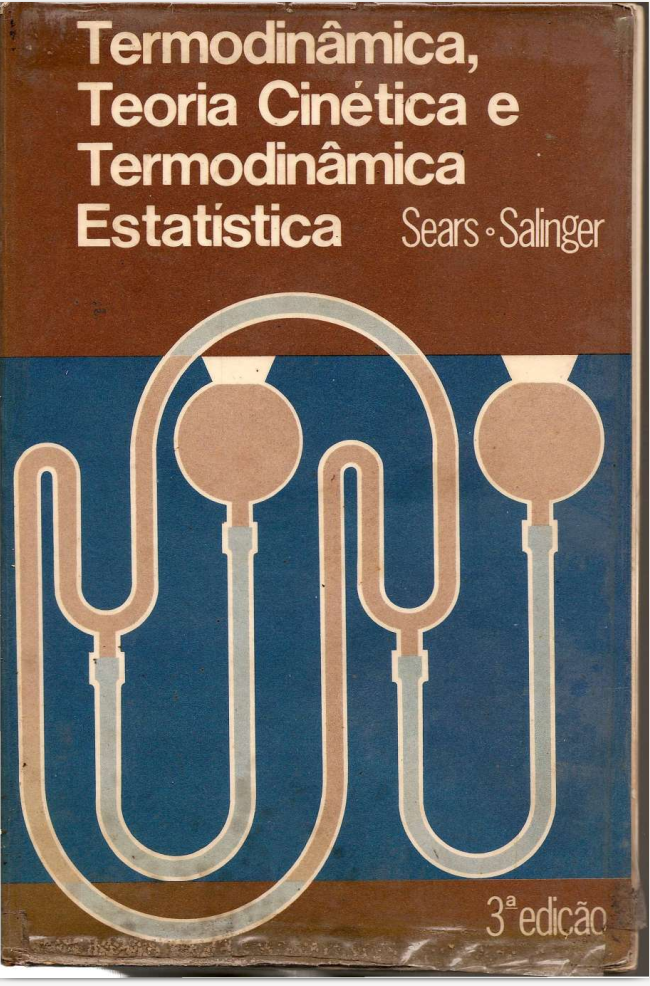
\includegraphics[height=0.8\textheight]{images/Captura de tela de 2023-03-27 07-48-28.png}
\end{frame}

\begin{frame}
    \centering
    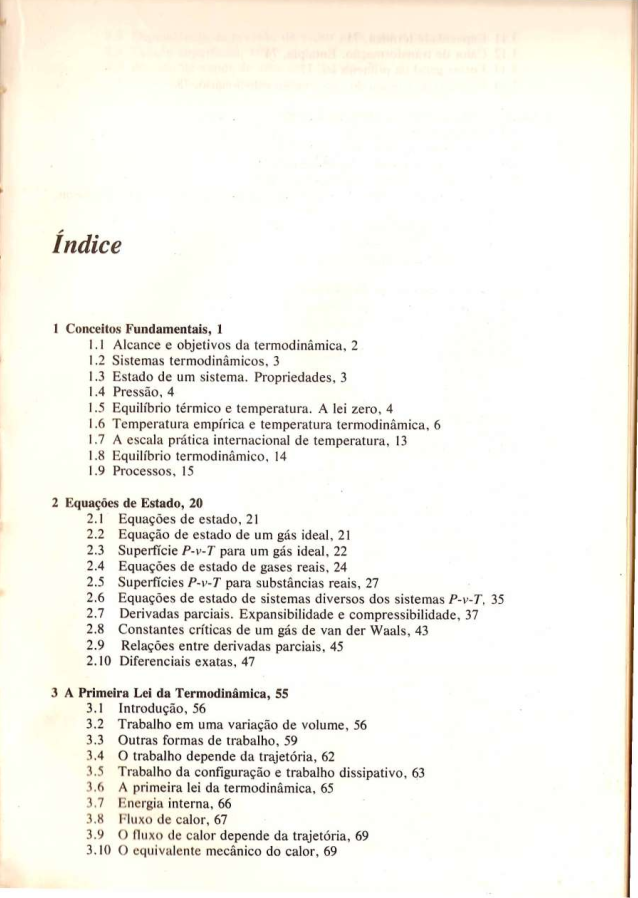
\includegraphics[width=0.32\textwidth]{images/Captura de tela de 2023-03-27 07-48-56.png}
    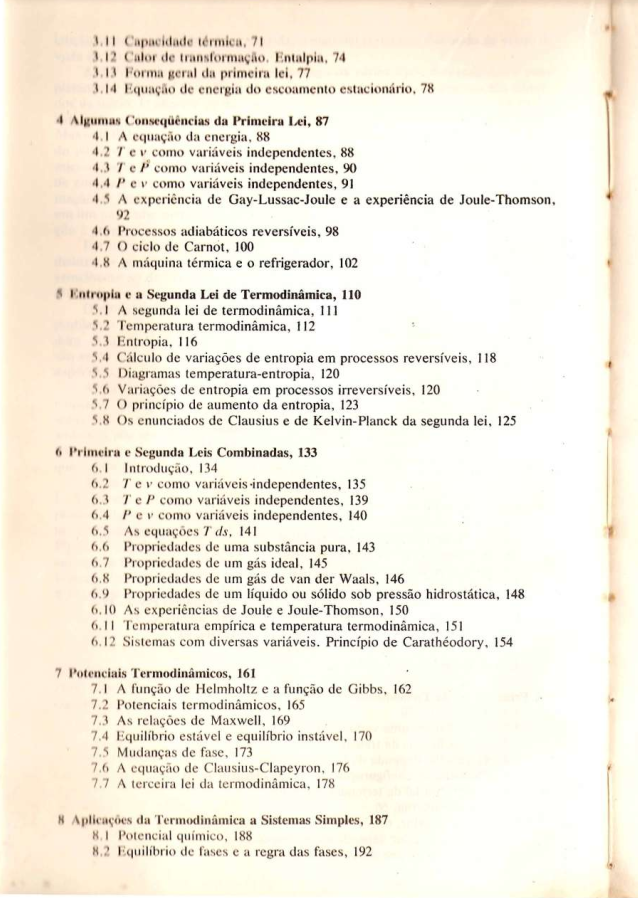
\includegraphics[width=0.32\textwidth]{images/Captura de tela de 2023-03-27 07-49-06.png}
    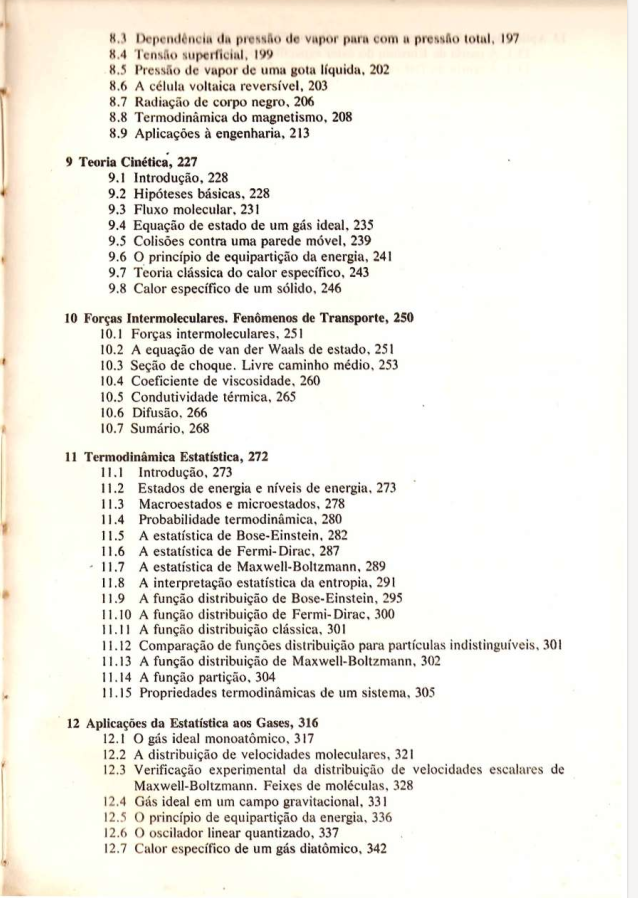
\includegraphics[width=0.32\textwidth]{images/Captura de tela de 2023-03-27 07-49-18.png}
\end{frame}

\againframe<2>{ementa}

\begin{frame}[c]{Termodinâmica}
    \begin{minipage}{\textwidth}
        \color{blue}
        Se as teorias físicas fossem pessoas, a Termodinâmica seria a bruxa da
        aldeia. Ao longo de três séculos, ela sorriu silenciosamente enquanto
        outras teorias surgiam e desapareciam, sobrevivendo a grandes
        revoluções na Física, como o advento da relatividade geral e da
        mecânica quântica. As outras teorias a acham um tanto estranha, de
        alguma forma de natureza diferente do restante, mas todos vêm a ela em
        busca de conselhos e ninguém ousa contradizê-la. Einstein, por exemplo,
        chamou-a de “a única teoria física de conteúdo universal, que estou
        convencido de que dentro da estrutura de aplicabilidade de seus
        conceitos básicos nunca será derrubada”
    \end{minipage}

    \vspace{1cm}
    John Goold \textit{et al} 2016 J. Phys. A: Math. Theor. 49 143001 \\
    https://doi.org/10.1088/1751-8113/49/14/143001
\end{frame}

\begin{frame}[c]{Leis da Termodinâmica, versão poltrona do vovô}
    \begin{itemize}
        \item Lei zero: Se você tocar em alguma coisa, você entra no jogo
        \item Lei um: A vida é um jogo
        \item Lei dois: Você não pode vencer
        \item Lei três: Você não pode nem empatar
    \end{itemize}

    \vspace{1cm}
    Escrito por Thomas Tabb Mayo IV
\end{frame}

\begin{frame}[c]{Mecânica Estatística}
    \begin{minipage}{\textwidth}
        \color{blue}
        Ludwig Boltzmann, who spent much of his life studying statistical
        mechanics, died in 1906, by his own hand. Paul Ehrenfest, carrying on the
        work, died similarly in 1933. Now it is our turn to study statistical
        mechanics.
    \end{minipage}

    \vspace{1cm}
    Texto de David L. Goodstein no livro \textit{States of Matter} (1975)
\end{frame}

\begin{frame}{Então...}
    \begin{itemize}
        \item A Termodinâmica é uma ciência experimental, baseada em um pequeno
            número de princípios, que são generalizações feitas a partir da
            experiência
        \item \textcolor{red}{Ela trabalha apenas com as propriedades \textit{macroscópicas} da
            matéria}
        \item Dos princípios da termodinâmica podemos obter relações gerais
            entre grandezas físicas e como essas dependem da temperatura.
        \item Os princípios da termodinâmica nos dizem quais as relações entre as 
            grandezas físicas que devem ser experimentalmente determinadas para que 
            \textit{todas} as propriedades do sistema sejam \textit{completamente} determinadas
    \end{itemize}
\end{frame}

\begin{frame}{Sistema}
    \begin{itemize}
        \item \textbf{Sistema} é tudo aquilo que queremos estudar. Ele pode ser tão simples 
            como um corpo livre (por exemplo, uma manga caindo de uma árvore) ou tão complexo como
            um motor de combustão
        \item Tudo que é externo ao sistema é considerado parte das \textbf{vizinhanças} do sistema
        \item Um sistema \textbf{fechado} sempre contém a mesma quantidade de matéria, ou seja, 
            não pode ocorrer troca de matéria com a sua vizinhança
        \item Um sistema \textbf{isolado} é um sistema fechado que não interage de forma alguma
            com a sua vizinhança
        \item O \textbf{estado} de um sistema é especificado pelos valores de certas grandezas
            mensuráveis experimentalmente chamadas \textit{variáveis de estado} ou \textit{propriedades}
        \item Exemplos de propriedades são a temperatura, a pressão exercida e o volume ocupado
        \item Note que a energia transferida entre o sistema e sua vizinhança não é uma propriedade
        \item Quando qualquer propriedade de um sistema varia, o estado do sistema varia e diz-se que o 
            sistema está sofrendo um \textbf{processo}
    \end{itemize}
\end{frame}

\begin{frame}{Um processo, dois sistemas...}
    \begin{minipage}{\textwidth}
        Ar está contido em um conjunto cilindro-pistão vertical equipado com uma resistência
        elétrica. A atmosfera exerce uma pressão de \SI{101.3}{kPa} no topo do pistão, que possui
        uma massa de \SI{45.4}{kg} e cuja área da face é de \(\SI{0.09}{m^2}\). Uma corrente 
        elétrica passa através da resistência e o volume aumenta lentamente de \(\SI{0.04}{m^3}\),
        enquanto sua pressão permanece constante. A massa do ar é \SI{0.27}{kg} e sua \textbf{energia interna}
        específica aumenta de \SI{41.9}{kJ/kg}. O ar e o pistão estão em repouso no início e fim do processo.
        O material do cilindro-pistão é um bom isolante. O atrito entre o pistão e a parede do cilindro pode ser 
        desprezado, e a aceleração da gravidade é \(g=\SI{9.7}{m/s^2}\).
    \end{minipage}
    \begin{enumerate}[(a)]
        \item Para um sistema composto de apenas ar, determine a transferência de \textbf{calor} da resistência para o ar 
            e o \textbf{trabalho} realizado \textit{pelo} sistema
        \item Para um sistema composto de ar e pistão, determine a transferência de calor da resistência para o ar 
            e o trabalho realizado pelo sistema
    \end{enumerate}

    \pause

    \begin{tcolorbox}[colback=red!20]
        O que é energia interna, calor e trabalho? Como essas grandezas se relacionam?
    \end{tcolorbox}
\end{frame}

\begin{frame}[c]
    \centering
    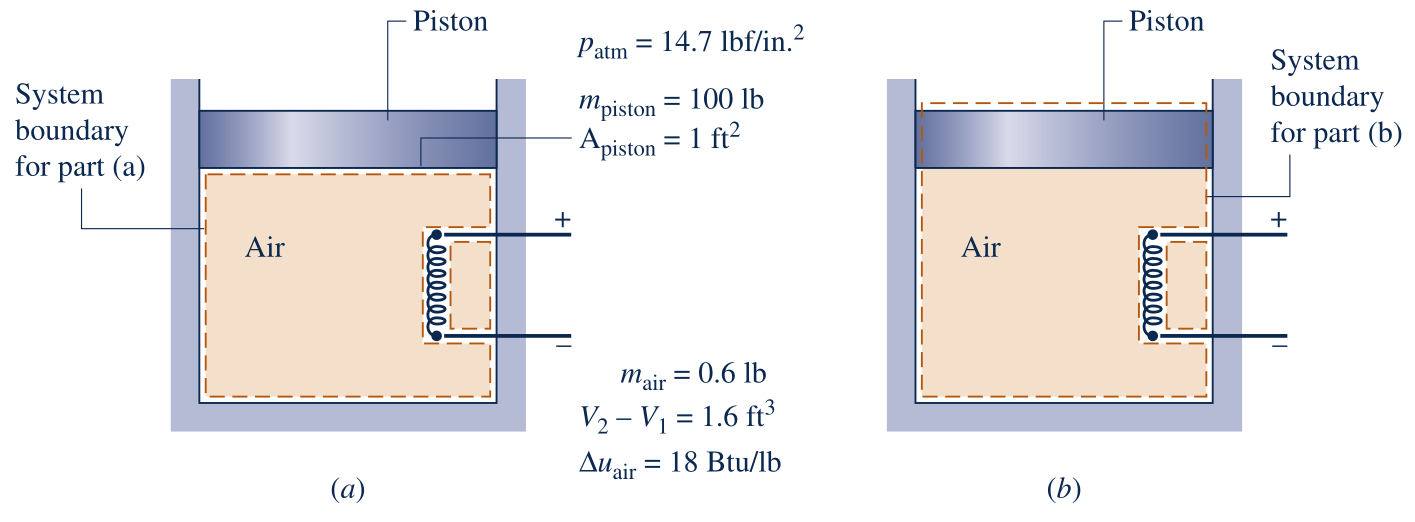
\includegraphics[width=0.9\textwidth]{images/Captura de tela de 2023-03-29 08-03-41.png}
\end{frame}

\begin{frame}{Observações}
    \begin{itemize}
        \item Uma grandeza é uma propriedade se, e somente se, sua mudança de valor
            entre dois estados é independente do processo
        \item Ou seja, se o valor de uma determinada grandeza depende dos detalhes do
            processo e não apenas dos estados extremos, essa grandeza não pode ser uma propriedade
        \item Um sistema está em \textbf{equilíbrio} quando não há mudanças no valor de suas propriedades 
            \textit{após ser isolado}
    \end{itemize}
    \centering
    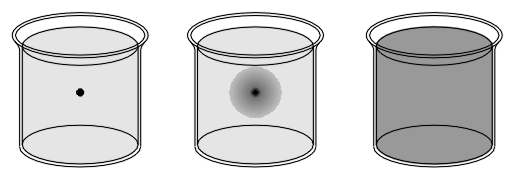
\includegraphics[width=0.8\textwidth]{images/termo4.png}
\end{frame}

\begin{frame}{Pergunta difícil}
    \begin{minipage}{\textwidth}
        Uma mistura de hidrogênio e oxigênio é isolada e deixada alcançar um estado de temperatura 
        e pressão constantes. A mistura é explodida com uma centelha de energia desprezível e novamente
        deixada atingir um estado de temperatura e pressão constantes
    \end{minipage}
    \begin{enumerate}
        \item O estado inicial é um estado de equilíbrio? Explique
        \item O estado final é um estado de equilíbrio? Explique
    \end{enumerate}
\end{frame}

\begin{frame}{Princípio dos estados equivalentes}
\begin{itemize}
    \item Existe uma propriedade \textit{intensiva} independente para cada forma pela qual a energia de um sistema pode ser variada independentemente 
    \item Formas de transferência de energia: calor + trabalho (várias formas)
    \item Ou seja: o número de propriedades \textit{intensiva} independentes é igual  ao número de interações relevantes do sistema devido a trabalho mais um (calor)
\end{itemize}
\begin{block}
    {Sistema compressível simples}
    \begin{itemize}
        \item \textbf{Sistema simples}: existe somente uma forma pela qual a energia do sistema pode ser significativamente alterada por trabalho
        \item \textbf{Sistema compressível simples}: o trabalho é relacionado a uma mudança no volume
        \item Em um sistema compressível simples, a temperatura e o volume específico podem ser considerados independentes e a pressão como função destes dois, ou seja, 
        \(
        P= P(T,v)
        \)
        \item Dessa função temos uma superfície \(P-v-T\)
    \end{itemize}
\end{block}
\end{frame}

\begin{frame}{Superfície P-v-T da água\footnote{possivelmente}}
\centering
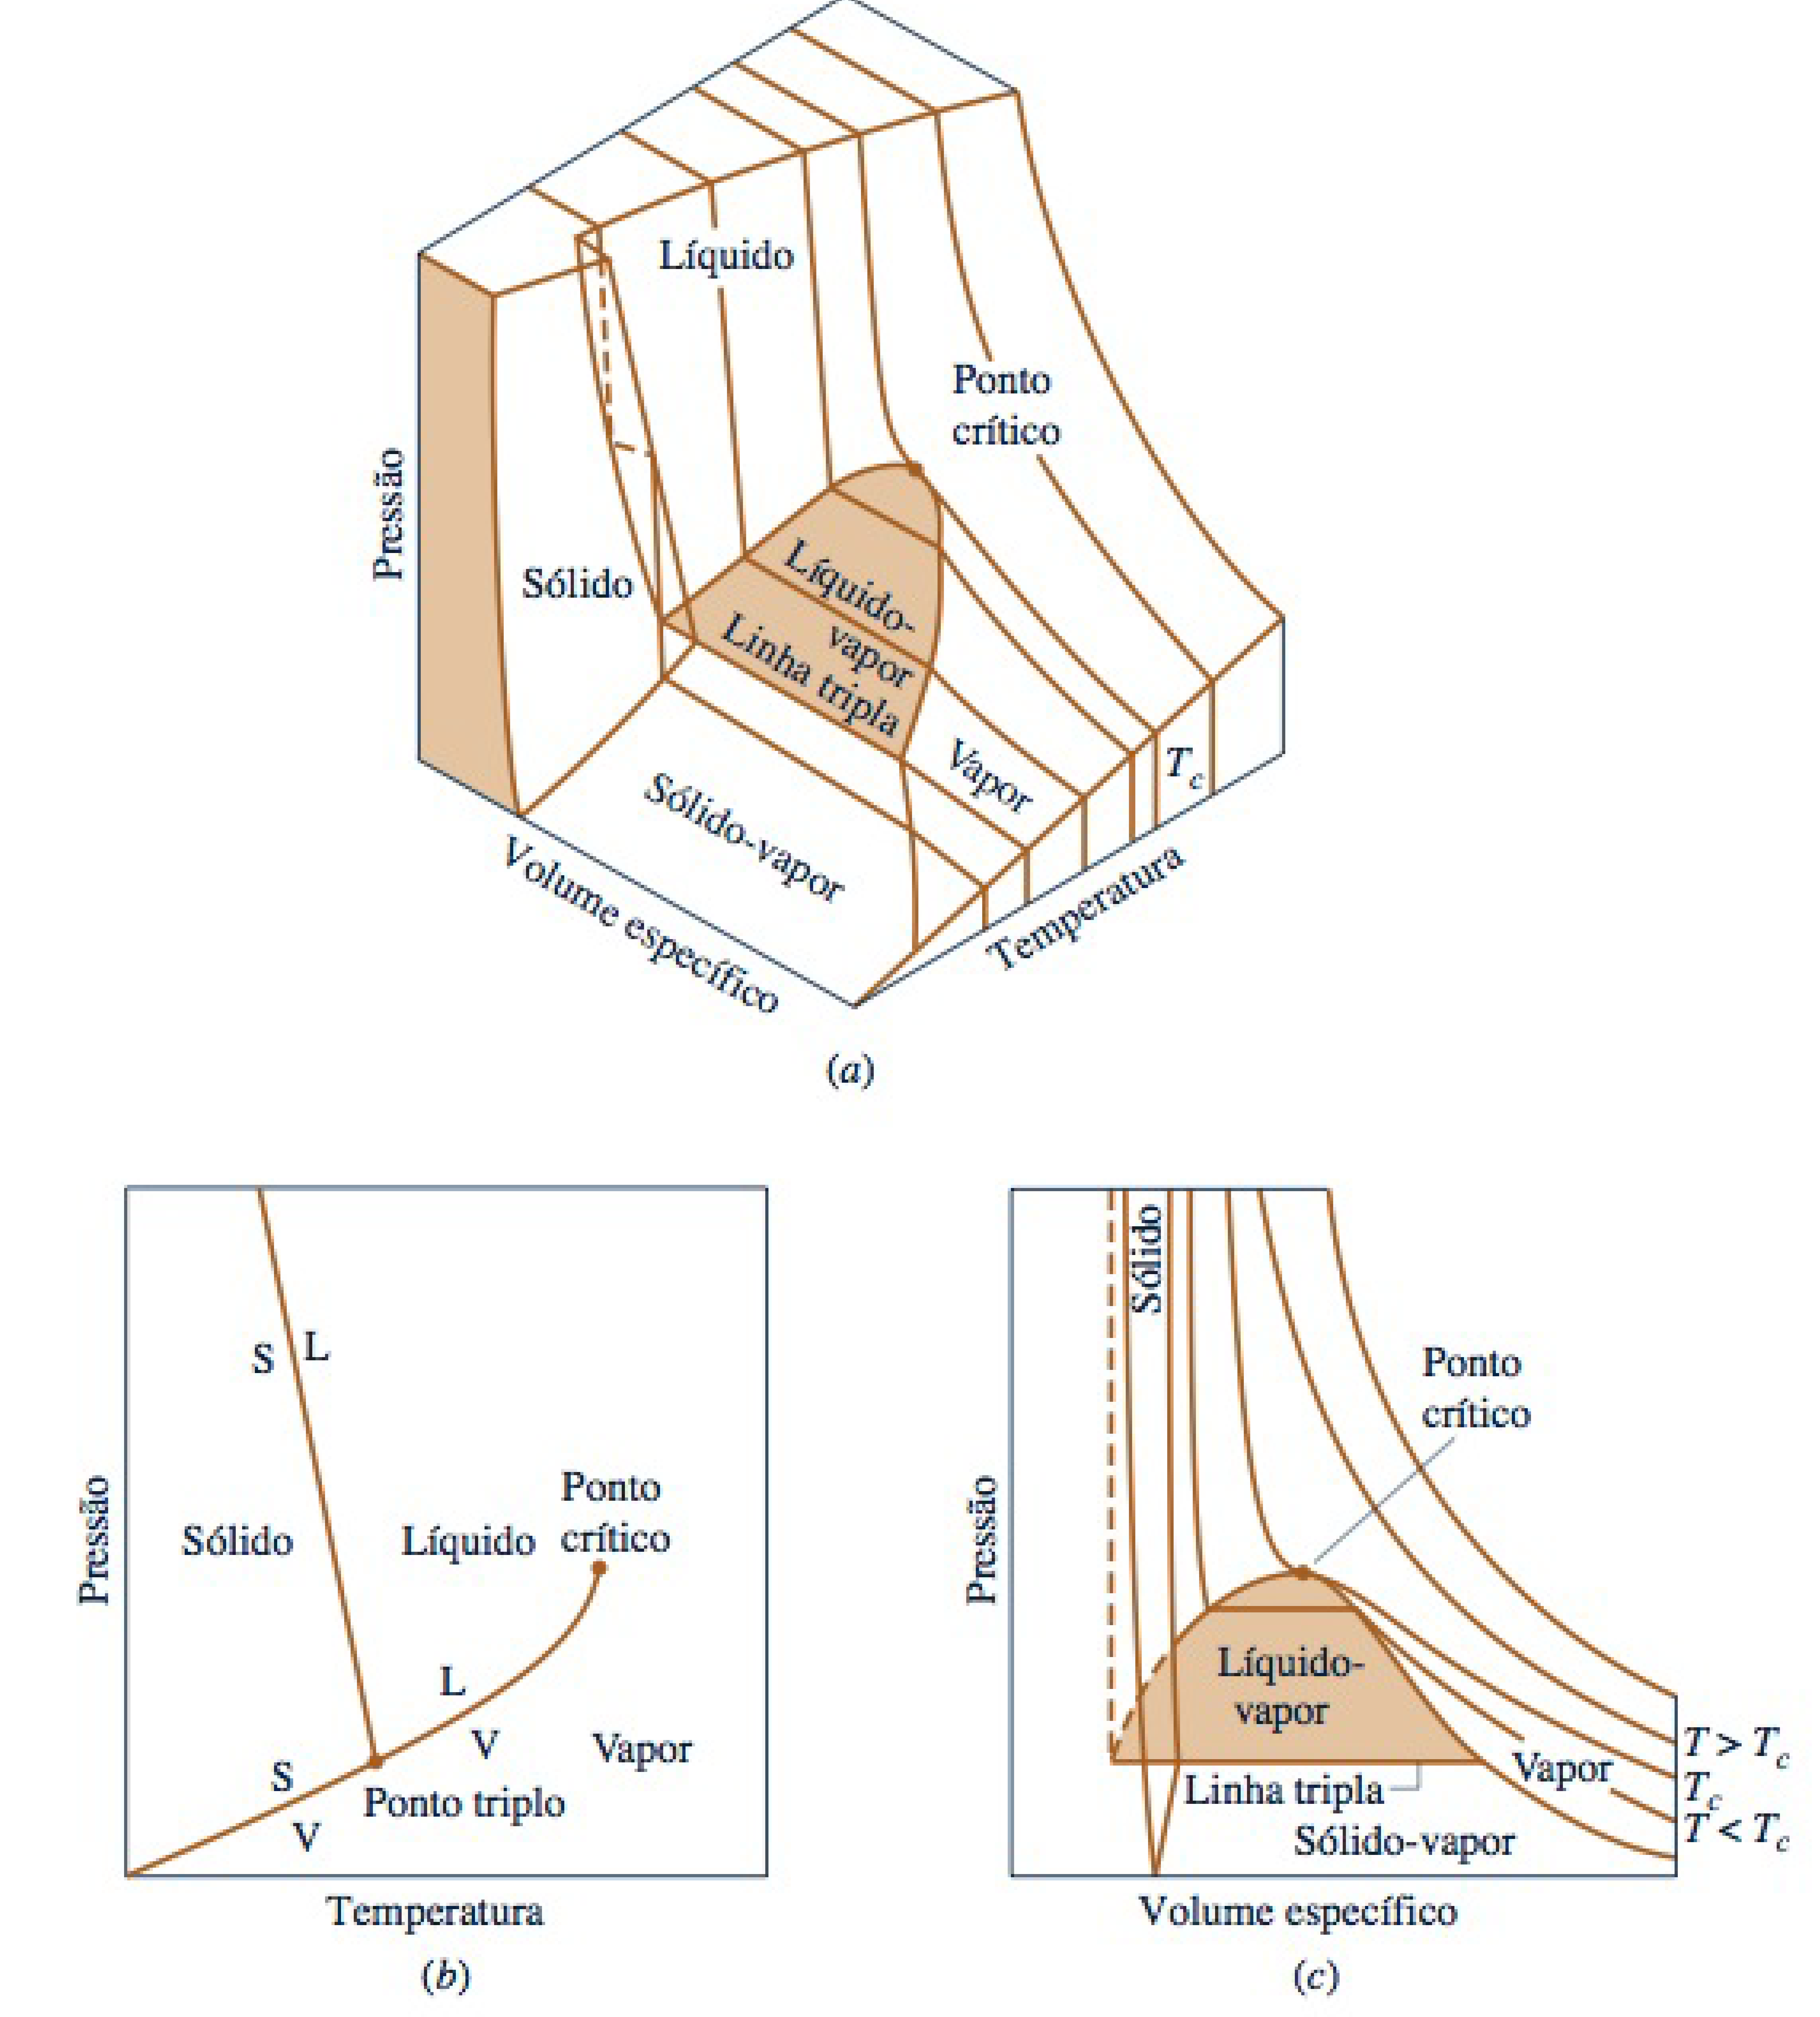
\includegraphics[height=7.5cm-5pt]{images/pvt.png}
\end{frame}

\begin{frame}{Gás ideal}
\[
    Pv = RT \leftarrow \text{equação de estado}
\]
\centering
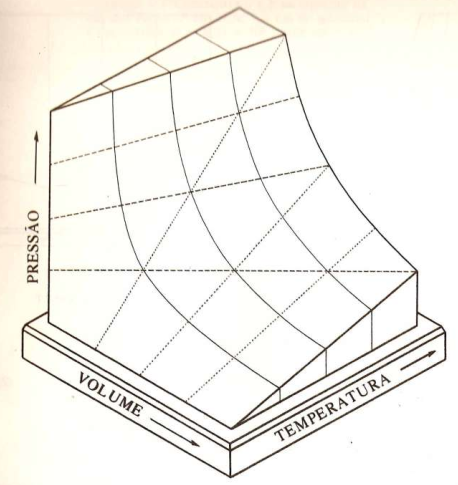
\includegraphics[height=7.5cm-60pt]{images/pvt-ideal.png}

\pause

\(R=\SI{8.3143e3}{\dfrac{J}{kmol~K}}\) é a constante \textbf{universal} dos gases 
\end{frame}

\begin{frame}
    \centering
    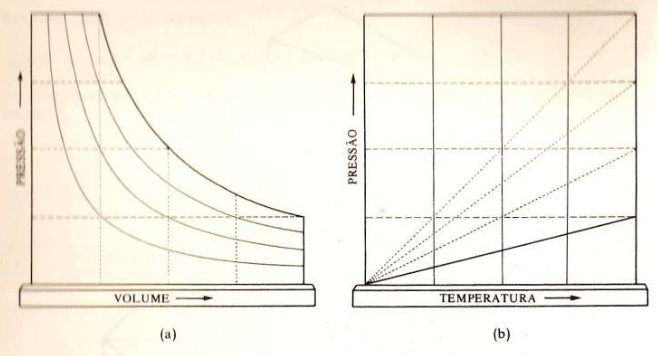
\includegraphics[height=0.8\textheight]{images/Captura de tela de 2023-04-03 13-42-22.png}
    \begin{columns}
        \begin{column}{0.4\textwidth}
            \[
                \textcolor{blue}{P}=R\frac{T}{\textcolor{red}{v}}
            \]
        \end{column}

        \begin{column}{0.4\textwidth}
            \[
                \textcolor{blue}{P}=R\frac{\textcolor{red}{T}}{v}
            \]
        \end{column}
    \end{columns}
\end{frame}

\begin{frame}[c]{Gases de van der Waals}
\[
    \left(P+\frac{a}{v^2}\right)(v-b)=RT
\]

\centering
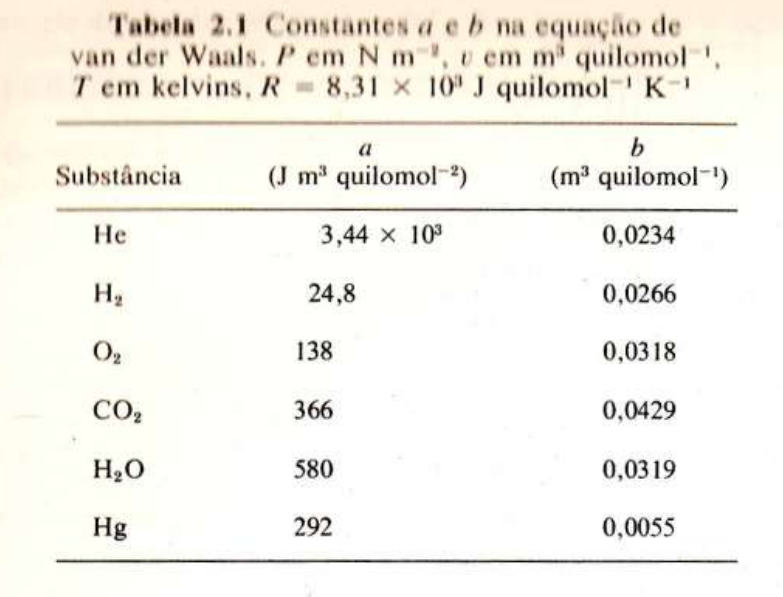
\includegraphics[height=\textheight-70pt]{images/Captura de tela de 2023-04-12 07-51-46.png}
\end{frame}

% \begin{frame}[c]
%     \begin{columns}[T]
%         \begin{column}{0.4\textwidth}
%             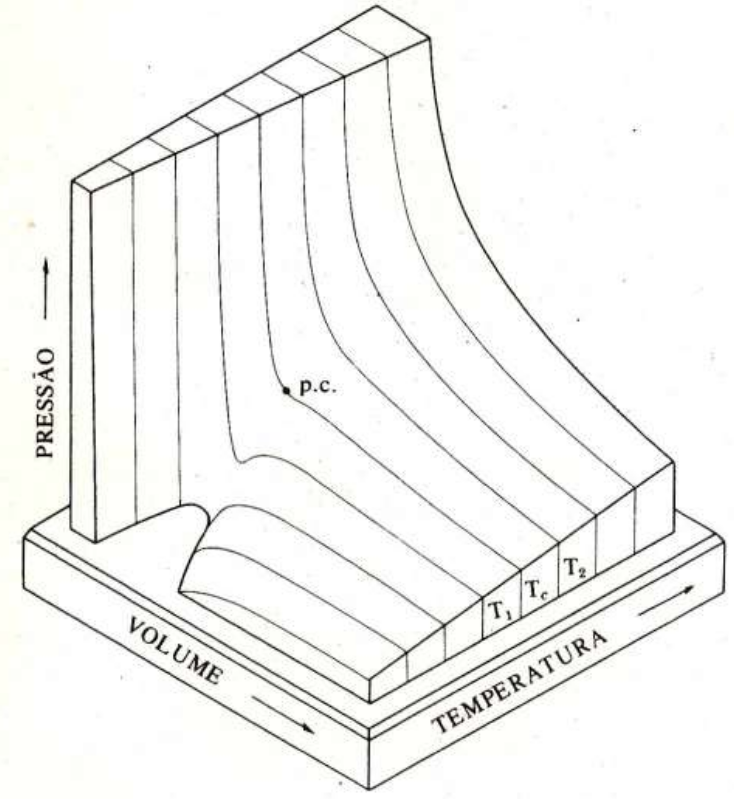
\includegraphics[width=\textwidth]{images/Captura de tela de 2023-04-12 08-15-26.png}
%         \end{column}

%         \begin{column}{0.4\textwidth}
%             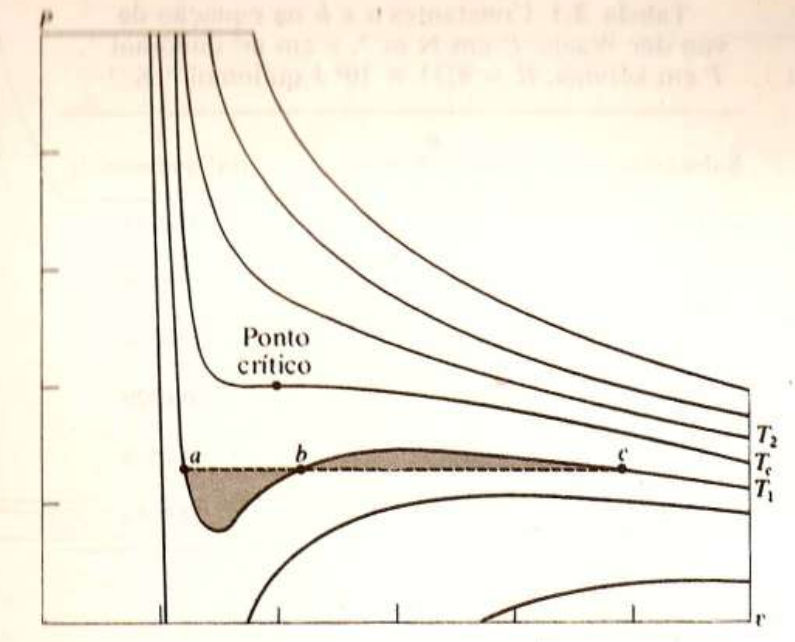
\includegraphics[width=\textwidth]{images/Captura de tela de 2023-04-12 08-17-41.png}
%         \end{column}
%     \end{columns}
%     \pause
% \end{frame}

% \begin{frame}{Substância real: \(\text{CO}_2\)}
%     \begin{center}
%         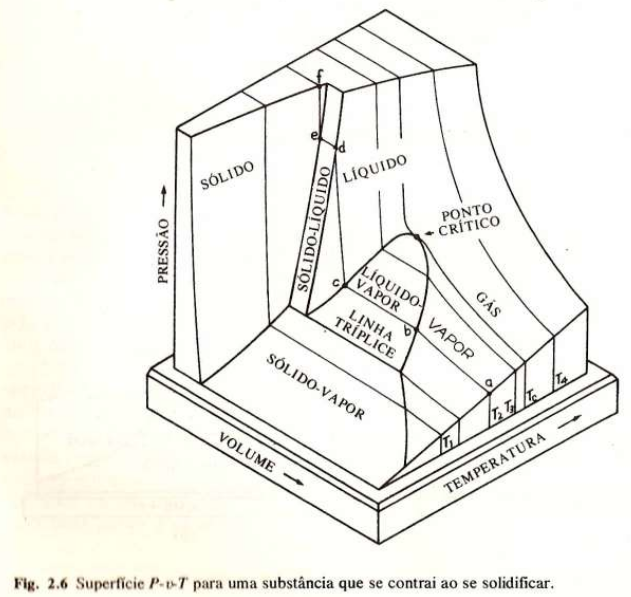
\includegraphics[height=\textheight-35pt]{images/Captura de tela de 2023-04-12 08-40-12.png}
%     \end{center}
% \end{frame}

\begin{frame}[c]{Equação de estado para um fio sob tensão}
    \[
        L=L_0 \left[ 1+ \frac{\mathcal{F}}{YA}+\alpha (T-T_0) \right]
    \]
    onde 
    \begin{itemize}
        \item \(L\) é o comprimento do fio
        \item \(L_0\) é o comprimento sob tensão nula à temperatura \(T_0\)
        \item \(Y\) é o módulo de Young (\textit{propriedade relacionada a elasticidade})
        \item \(A\) é a área da seção reta
        \item \(\alpha\) é o coeficiente de dilatação linear
        \item \(\mathcal{F}\) é a tensão
    \end{itemize}
\end{frame}

\begin{frame}{Cálculo...}
    \begin{itemize}
        \item A equação de estado de um sistema \(PVT\)\footnote{\(v\) e \(V\) são diferentes, por quê?} 
            é uma relação entre \(P\), \(V\) e \(T\) em qualquer estado de equilíbrio do sistema
        \item Há muitas outras propriedades no sistema e, possivelmente, outras equações de estado
        \item O \textit{coeficiente de dilatação volumétrica} de um material é definido como
            \[
                \beta \equiv \frac{1}{V}\left(\frac{\partial V}{\partial T}\right)_P
            \]
        \item O \textit{coeficiente de compressão isotérmica} de um material é definido como
            \[
                \kappa \equiv -\frac{1}{V}\left(\frac{\partial V}{\partial P}\right)_T
            \]
        \item Como vimos em Cálculo, se \(V\)\footnote{na verdade, \(v\)...} é uma propriedade e \(V=V(P,T)\), temos
            \[
                dV = \frac{\partial V}{\partial T} dT + \frac{\partial V}{\partial P} dP 
                \implies dv = \beta V dT - \kappa V dP
            \]
    \end{itemize}
\end{frame}

\begin{frame}
    \begin{itemize}
        \item Se a equação anterior for integrada de algum estado de referência
            \(V_0\), \(P_0\), \(T_0\) até algum estado arbitrário
            \(V\), \(P\), \(T\) obteremos
            \[
                \int_{V_0}^V = V-V_0 = \int_{T_0}^T \beta V dT
                - \int_{P_0}^P \kappa V dP
            \]
        \item \textcolor{red}{Considerando} \(V\) constante  quando \(P\) e \(T\)
            são variadas e, além disso, \(\beta\) e \(\kappa\) também
            constantes, temos que
            \[
                V=V_0 [ 1+\beta (T-T_0) - \kappa (P-P_0)]
            \]
            \textcolor{red}{ou seja, é possível obter a equação de estado de um sólido ou líquido}
    \end{itemize}
\end{frame}

\begin{frame}{Exercício 2-14}
    \centering
    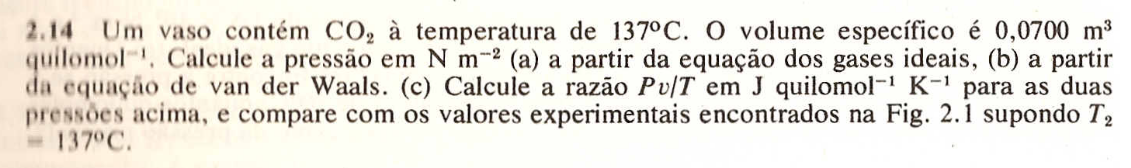
\includegraphics[width=\textwidth]{images/Captura de tela de 2023-04-12 13-20-49.png} \\
    \begin{columns}[c]
        \begin{column}{\textwidth-20ex}
            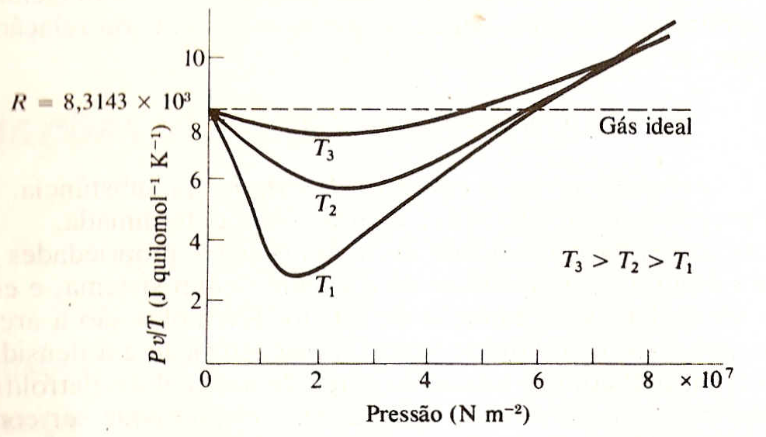
\includegraphics[height=\textheight-93pt-2pt]{images/Captura de tela de 2023-04-12 13-23-51.png}
        \end{column}
        \begin{column}{20ex}
            Figura 2.1
        \end{column}
    \end{columns}
\end{frame}

\begin{frame}{Exercícios 2-17 e 2-18}
    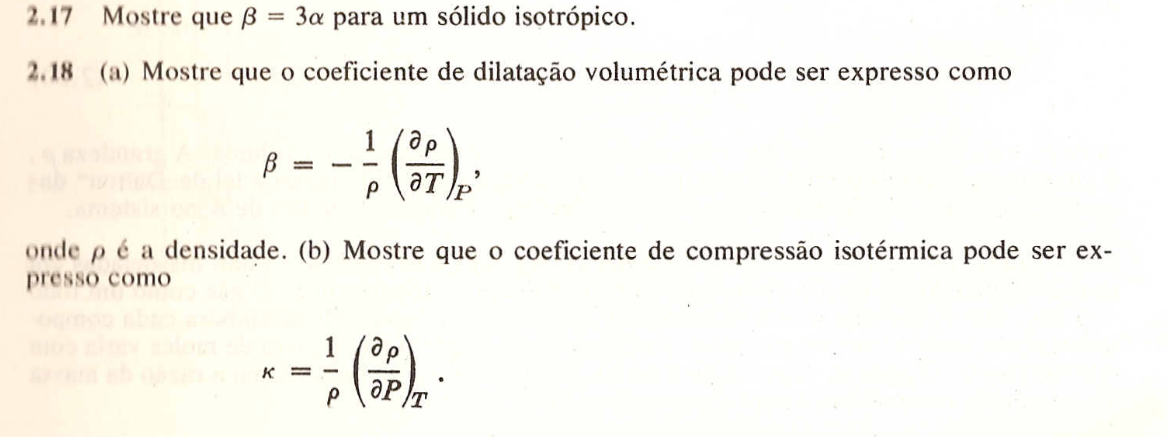
\includegraphics[width=\textwidth]{images/Captura de tela de 2023-04-12 13-41-26.png}
\end{frame}

\begin{frame}{Trabalho na termodinâmica}
    \centering
    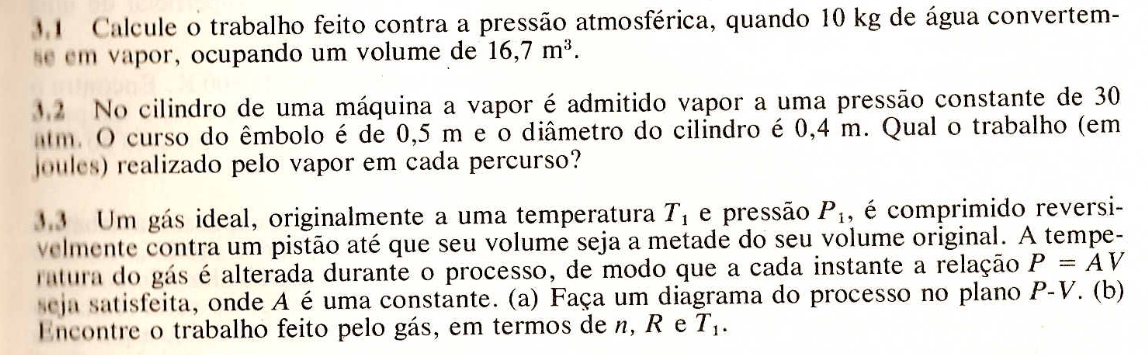
\includegraphics[width=\textwidth]{images/Captura de tela de 2023-04-17 13-42-39.png}

    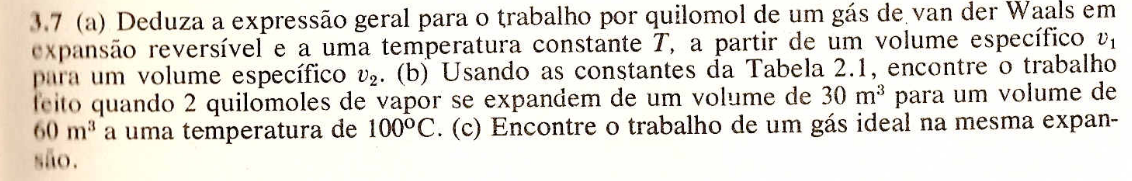
\includegraphics[width=\textwidth]{images/Captura de tela de 2023-04-17 13-57-07.png}
\end{frame}

\begin{frame}{Diferenciais exatas}
    \begin{itemize}
        \item Sejam
            \begin{gather*}
                dV_{1-2-3} = \left(\frac{\partial V}{\partial T}\right)_{P_1}dT+
                \left(\frac{\partial V}{\partial P}\right)_{T_2}dP \\
                dV_{1-4-3} = \left(\frac{\partial V}{\partial T}\right)_{P_3}dT+
                \left(\frac{\partial V}{\partial P}\right)_{T_1}dP
            \end{gather*}
            \only<2->{
            \item Subtraindo, temos
                \[
                    \frac{
                        \left(\frac{\partial V}{\partial T}\right)_{P_3}-
                        \left(\frac{\partial V}{\partial T}\right)_{P_1}
                    }{dP} =
                    \frac{
                        \left(\frac{\partial V}{\partial P}\right)_{T_2}-
                        \left(\frac{\partial V}{\partial P}\right)_{T_1}
                    }{dT} 
                \]
                ou seja,
                \[
                    \frac{\partial^2 V}{\partial P \partial T} = 
                    \frac{\partial^2 V}{\partial T \partial P} 
                \]
            \item O valor da segunda derivada parcial mista é independente da ordem de derivação
            \item Ou seja, \(dV\) é uma diferencial exata \textbf{e uma propriedade termodinâmica}
            }
    \end{itemize}
    \only<1>{
        \begin{center}
            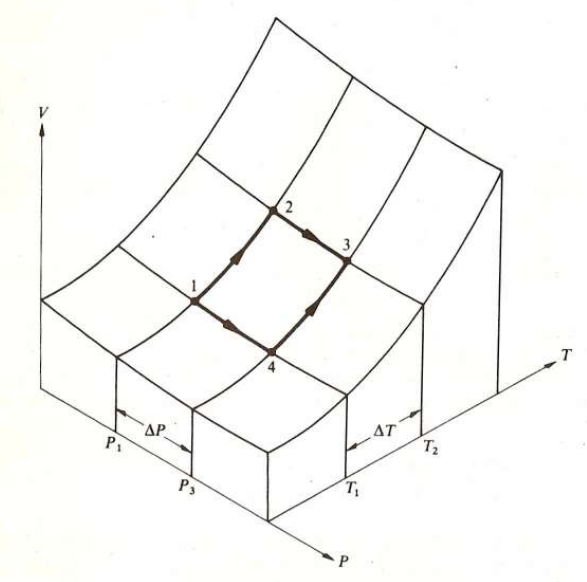
\includegraphics[height=\textheight-115pt]{images/Captura de tela de 2023-04-26 08-27-55.png}
        \end{center}
    }
\end{frame}

\begin{frame}
    \begin{tcolorbox}[colback=red!10]
        \begin{itemize}
            \item Calor e trabalho não são propriedades (dependem do processo) e, portanto, ''pequenas quantidades''
                dessas grandezas não são diferenciais exatas
            \item Por exemplo, o trabalho realizado em 1-2-3 é diferente do realizado em 1-4-3
            \item Por isso, representamos de uma forma diferente: \(d'Q\) e \(d'W\)

                \centering
                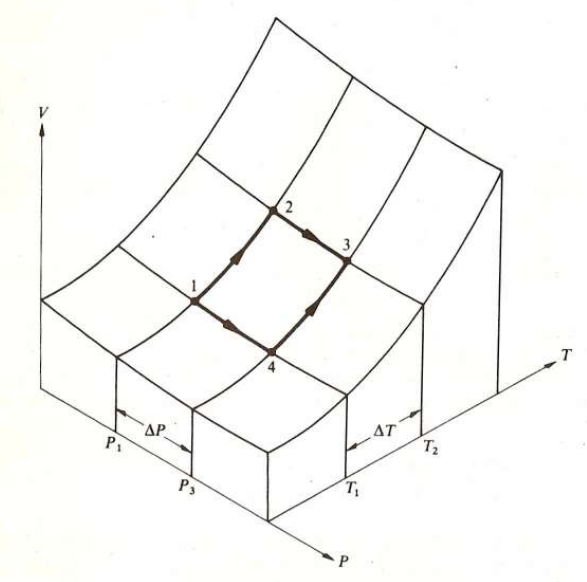
\includegraphics[height=\textheight-88pt]{images/Captura de tela de 2023-04-26 08-27-55.png}
        \end{itemize}
    \end{tcolorbox}
\end{frame}

\begin{frame}{Forma diferencial da primeira lei da termodinâmica}
    \[
        \boxed{dU = d'Q - d'W}
    \]
\begin{itemize}
    \item \textit{Para um sistema compressível simples e processos reversíveis}, podemos escrever
        \[
            dU=d'Q-PdV
        \]
    \item Em muitas ocasiões, principalmente na \textit{Química}, a quantidade
        \(U+PV\) aparece e chamamos ela de \textbf{entalpia} (ver seção 3.12 para mais detalhes)
        \[
            dH = d'Q+VdP
        \]
    \item \textcolor{red}{Letras são importantes}: da mecânica clássica temos que \(E=K+U\), onde \(K\)
        é a energia cinética e \(U\) a energia potencial. \textbf{Mas}, em termodinâmica, \(U\) é
        energia interna... Assim, temos as seguintes equações diferentes tratando da ''mesma coisa''
        \[
            \Delta U = Q-W \qquad \Delta U = Q+W \qquad \Delta E = Q - W
        \]
        com a ''cereja do bolo'' \(W=\Delta K\), totalmente errada nesse contexto
\end{itemize}
\end{frame}

\begin{frame}{Ciclo de Carnot e definição de temperatura}
    \begin{itemize}
        \item Na seção 4.7, podemos ver a demonstração da equação 4-47
            \[
                \frac{Q_2}{Q_1} = \frac{T_2}{T_1} \tikzmark{bup}
            \]
            \textit{para um gás ideal}
        \item Mas, \textit{conforme pode ser visto na seção 5.2}, 
            \[
                \frac{Q_2}{Q_1} = \frac{\phi(\theta_2)}{\phi(\theta_1)}
            \]
            onde \(\theta_2\) e \(\theta_1\) são temperaturas
        \item Definindo \(T=A\phi(\theta)\), temos
            \[
                \frac{Q_2}{Q_1} = \frac{T_2}{T_1} \implies T=T_3 \frac{Q_2}{Q_1}
            \]
            e com isso temos a definição de temperatura, ''sem o uso de termômetro'' \tikzmark{bop}

            \only<2>{
                \tikz[remember picture, overlay] \draw [red,->] (pic cs:bop) to[out=0,in=0] ([yshift=1ex] pic cs:bup);
            }
    \end{itemize}
\end{frame}

\begin{frame}{Entropia}
    \begin{itemize}
        \item Temos que os valores de \(Q_1\) e \(Q_2\) vistos anteriormente estão em \textit{módulo}
            e, usando os valores com sinal, teríamos
            \[
                \frac{T_2}{T_1}=-\frac{Q_2}{Q_1} \implies \frac{Q_1}{T_1} + \frac{Q_2}{T_2}=0
            \]
            \begin{center}
                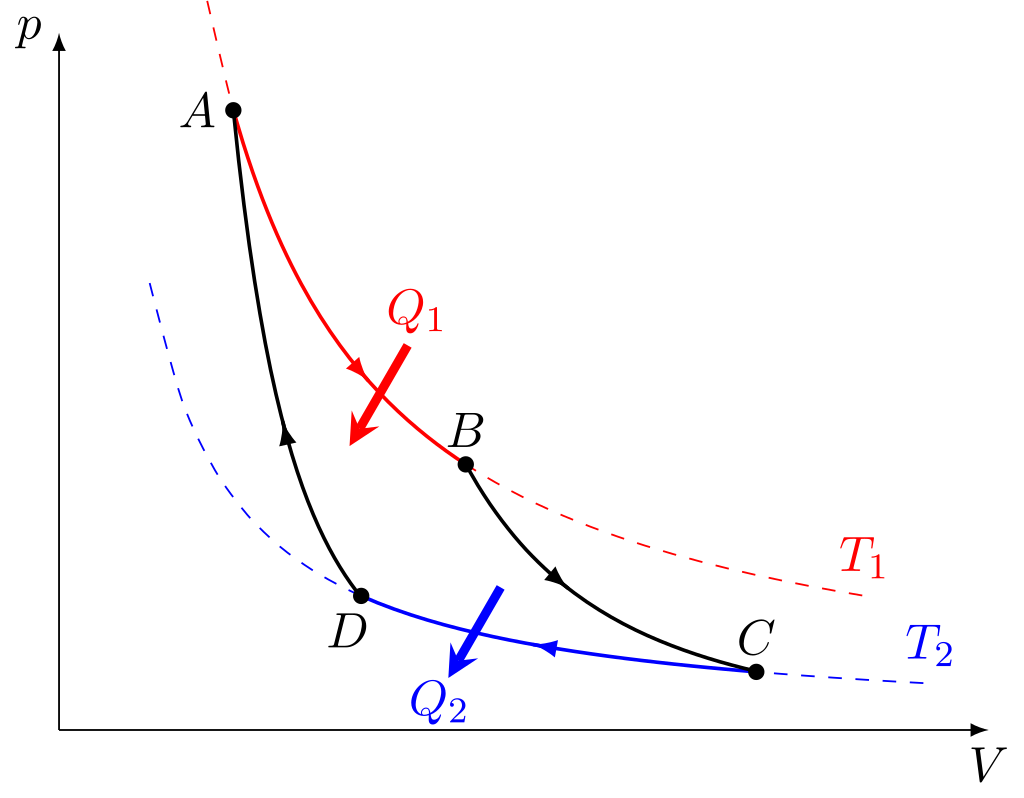
\includegraphics[height=\textheight-92pt-42pt]{images/Carnot-cycle-p-V-diagram.svg.png}
            \end{center}
        \item O resultado líquido de um processo \textit{reversível} cíclico pode ser 
            aproximado, tão de perto quanto se queira, por um grande número de ciclos de Carnot,
            todos percorridos no mesmo sentido
    \end{itemize}
\end{frame}

\begin{frame}
    \begin{itemize}
        \item Ou seja
            \[
                \oint {\frac{d'Q_r}{T}} = 0
            \]
            onde o índice \(r\) indica que se trata de um processo reversível
        \item Assim, apesar de \(d'Q\) não ser uma diferencial exata, a razão \(d'Q/T\) é
        \item Assim, podemos definir uma propriedade chamada \textbf{entropia}, onde
            \[
                dS \equiv \frac{d'Q}{T}
            \]
        \item Independente do processo que leve um estado \(a\) a um estado \(b\), temos 
            \[
                \int_{a}^{b} dS=S_b - S_a = \Delta S
            \]
        \item Para um processo cíclico reversível, temos \(\Delta S=0\)
        \item A entropia de um sistema é determinada \textit{a menos de uma constante arbitrária}

    \end{itemize}
\end{frame}

\begin{frame}{Cálculo de \(\Delta S\)}
    \begin{itemize}
        \item Para um processo adiabático:
        \item Para um processo isotérmico:
        \item<3-> Para um processo a pressão/volume constante:
        \item<4-> Resolva a questão 5.12
    \end{itemize}
    \begin{center}
        \includegraphics<2>[height=\textheight-80pt-12pt]{images/Captura de tela de 2023-05-08 13-42-22.png}
        \includegraphics<4>[width=\textwidth]{images/Captura de tela de 2023-05-08 13-51-38.png}
    \end{center}
\end{frame}

\begin{frame}{O princípio do aumento da entropia}
    \begin{center}
        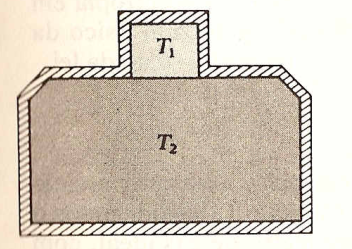
\includegraphics[height=\textheight-135pt]{images/Captura de tela de 2023-05-15 11-53-00.png}
    \end{center}
    \begin{itemize}
        \only<1>{
            \item Seja o processo apresentado na figura acima, onde a temperatura de
                um corpo é aumentada de \(T_1\) para \(T_2\) por contato do corpo com
                um único reservatório a uma temperatura \(T_2\)
            \item Se o processo se realizar a pressão constante e a capacidade térmica 
                puder ser considerada constante, então
                \[
                    \Delta S_\text{corpo} = C_P \ln{\frac{T_2}{T_1}}
                \]
            }
            \only<2>{
            \item Já o reservatório permanece com temperatura constante e o calor liberado
                pode ser calculado por
                \[
                    Q=C_P (T_2 - T_1)
                \]
                e 
                \[
                    \Delta S_\text{reservatório} = -\frac{Q}{T_2} = -C_P \frac{T_2-T_1}{T_2}
                \]
            }
            \only<3>{
            \item A variação total da entropia do sistema corpo+reservatório é dada por
                \[
                    \Delta S = \Delta S_\text{corpo}+\Delta S_\text{reservatório}=
                    C_P \left[\ln{\frac{T_2}{T_1}} - \frac{T_2-T_1}{T_2} \right]
                \]
            \item Fica como exercício mostrar que \(\Delta S\geq 0\)
            }
    \end{itemize}
\end{frame}

\begin{frame}
    \begin{itemize}
        \item Esse resultado é visto repetidamente na natureza: em todo processo
            que se realize em um sistema isolado, a entropia do sistema ou aumenta 
            (processo irreversível) ou permanece constante (processo reversível)
        \item Enquanto a ''energia nunca pode ser criada ou destruída'', a ''entropia não
            pode ser destruída, mas pode ser criada''
        \item Ou seja, os únicos estados que podem ser atingidos a partir de um dado
            estado inicial por processos adiabáticos são aqueles em que a entropia é
            maior ou igual à do estado inicial
        \item Resolva a questão 5.16
        \item Resolva a questão 5.21
    \end{itemize}
\end{frame}

\begin{frame}{Primeira e segunda leis combinadas}
    \begin{itemize}
        \item Temos que a primeira lei da termodinâmica na forma diferencial é dada por
            \[
                d'Q=dU+d'W
            \]
        \item Para um sistema \(PVT\), temos
            \[
                d'W=PdV
            \]
        \item A segunda lei ''define''
            \[
                dS = \frac{d'Q}{T}
            \]
        \item Assim, podemos escrever
            \[
                TdS=dU + PdV
            \]

    \end{itemize}
\end{frame}

\begin{frame}{Entalpia, Helmholtz e Gibbs}
    \begin{itemize}
        \item Além da energia interna \(U\), temos as seguintes \textit{funções}
            \begin{gather*}
                H=U+PV \\
                F=U-TS \\
                G=F+PV
            \end{gather*}
        \item O calor absorvido ou liberado durante uma mudança de fase (temperatura 
            e pressão constantes) é igual a diferença entre as entalpias do sistema
            nas duas fases
        \item Em um processo \textit{à temperatura e volume constantes}, temos que o 
            trabalho ''não PdV'' é menor que o decréscimo de \(F\)
        \item Em um processo \textit{à temperatura e pressão constantes}, temos que o 
            trabalho ''não PdV'' é menor que o decréscimo de \(G\)
        \item Como \(F\) e \(G\) são relacionadas \textit{à parcela da energia disponível para virar trabalho},
            elas são comumente chamadas de energias livres
    \end{itemize}
\end{frame}

\begin{frame}{Diferenciais}
    \begin{itemize}
        \item Se são propriedades, têm diferenciais exatas:
            \begin{gather*}
                dU = TdS - PdV \\
                dF = dU - TdS - SdT = -SdT - PdV \\
                dG= dF + PdV + VdP = -SdT + VdP \\
                dH = dU + PdV + VdP = TdS + VdP
            \end{gather*}
        \item E como vimos em Cálculo II:
            \[
                z=f(x,y) \implies dz = \frac{\partial z}{\partial x} dx + \frac{\partial z}{\partial y} dy
            \]
    \end{itemize}
\end{frame}

\begin{frame}
    \begin{itemize}
        \item Ou seja:
            \begin{align*}
                    & \left(\frac{\partial U}{\partial S}\right)_V = T \qquad & \left(\frac{\partial U}{\partial V}\right)_S = -P \\
                    & \left(\frac{\partial F}{\partial T}\right)_V = -S \qquad & \left(\frac{\partial F}{\partial V}\right)_T = -P \\
                    & \left(\frac{\partial G}{\partial T}\right)_P = -S \qquad & \left(\frac{\partial G}{\partial P}\right)_T = V \\
                    & \left(\frac{\partial H}{\partial S}\right)_P = T \qquad & \left(\frac{\partial H}{\partial P}\right)_S = V
            \end{align*}
        \item Lembrando de Física III:
            \[
                E_x = \frac{\partial \phi}{\partial x} \qquad
                E_y = \frac{\partial \phi}{\partial y} \qquad
                E_z = \frac{\partial \phi}{\partial z} 
            \]
        \item Chamamos as grandezas \(U\), \(H\), \(F\) e \(G\) de potenciais termodinâmicos
    \end{itemize}
\end{frame}

\begin{frame}[c]{Equação característica}
    \begin{itemize}
        \item A equação para um potencial termodinâmico em termos de \textit{variáveis características} é conhecida
            como equação característica
        \item \textbf{Todas as propriedades termodinâmicas podem ser obtidas pela derivação da equação característica}
        \item Atividade: 
            \begin{itemize}
                \item Relações de Maxwell
                \item Problema 7.3
                \item Problema 7.8
                \item Problema 7.8 com a expressão do problema 7.7
                \item Problema 7.10

            \end{itemize}
    \end{itemize}
\end{frame}
